
%% Creator David Li
% Modified matlab xsl latex template file to suit needs
% This LaTeX was auto-generated from an M-file by MATLAB.
% To make changes, update the M-file and republish this document.

\documentclass[12pt]{scrartcl}
\nonstopmode

\title{Matlab}
\usepackage[utf8]{inputenc}
\usepackage{graphicx}
\usepackage{epstopdf}
\usepackage{color}
\usepackage{xcolor}
\usepackage{amsmath}
\usepackage[ocgcolorlinks]{hyperref}
\usepackage{bookmark}
\usepackage[hmargin=2cm,vmargin=2.5cm]{geometry}
\usepackage{fancyhdr}
\usepackage{booktabs}
\sloppy
\definecolor{lightgray}{gray}{0.5}
% \definecolor{myText}{HTML}{2B2B2B}
\definecolor{fontColor}{HTML}{171717}
\setlength{\parindent}{0pt}

\makeindex

\usepackage{listings}
\definecolor{mygreen}{RGB}{28,172,0} % color values Red, Green, Blue
\definecolor{mylilas}{RGB}{170,55,241}
\lstset{language=Matlab,%
	%basicstyle=\color{red},
	breaklines=true,%
	morekeywords={matlab2tikz},
	keywordstyle=\color{blue},%
	morekeywords=[2]{1}, keywordstyle=[2]{\color{black}},
	identifierstyle=\color{black},%
	stringstyle=\color{mylilas},
	commentstyle=\color{mygreen},%
	showstringspaces=false,%without this there will be a symbol in the places where there is a space
	%numbers=left,%
	%numberstyle={\tiny \color{black}},% size of the numbers
	%numbersep=9pt, % this defines how far the numbers are from the text
	emph=[1]{for,end,break},emphstyle=[1]\color{red}, %some words to emphasise
	%emph=[2]{word1,word2}, emphstyle=[2]{style},  
    %captionpos=b,
    %caption={Matlab Code Snippet:},
}
\usepackage{tcolorbox}
\tcbuselibrary{listings}
\tcbuselibrary{breakable}
\usepackage{float}

\newtcblisting[auto counter,number within=section*]{matlaboutput}[2][]{sharp corners, breakable,
    fonttitle=\bfseries,colback=white, colframe=black!90, listing only, 
    listing options={language=Matlab, showstringspaces=false, breakatwhitespace=true, breaklines=true, tabsize=4}, 
    title=Matlab Output \thetcbcounter: #1} 
\begin{document}

\begin{center}
	\hrule
	\vspace{.4cm}
	{\textbf { \large ELEC 460 --- Control Theory II}}
\end{center}
{\textbf{Name:}\ David Li \hspace{\fill} \textbf{Student Number:} \ V00818631  \\
{\textbf{Due Date:} February 1, 2018, 11:30 AM \hspace{\fill} \textbf{Assignment}  3}\\
\hrule

    
    
%\section*{ELEC 460 Assignment 3}
%\begin{par}
%Textbook Questions from Ogata B-3-4, B-3-6, B-3-7, B-3-15, B-3-19 from the textbook.
%\end{par} \vspace{1em}
%
%\tableofcontents
%\newpage
%\begin{par}
%Pulse transfer function relates Z-transform of the output at the sampling instants to the Z- transform of the sampled input.
%\end{par} \vspace{1em}


\subsection*{B-3-4}



%\begin{par}
%Consider a transfer function system
%\end{par} \vspace{1em}
%\begin{par}
%$$ X(s)=\frac{s+3}{(s+1)(s+2)}$$
%\end{par} \vspace{1em}
%\begin{par}
%Obtain the pulse transfer function by two different methods
%\end{par} \vspace{1em}
%\begin{lstlisting}[language = Matlab,frame=single,caption={}]
%syms s z
%B34Xs = (s+3)/((s+1)*(s+2))
%% First answer, ignore
%% B34XzA1 = subs(B34Xs ,s,z)
%% First answer, get the CTS function and convert that
%% to the Z-domain,
%XsTemp = ilaplace(B34Xs)
%B34XzA2 = ztrans(XsTemp)
%
%% Second Answer, convert from laplace domain to z domain using tables
%% will need to use partial fractions
%Xs2 = partfrac(B34Xs)
%% Using the tables
%% Answer is the same
%\end{lstlisting}
%
% \begin{matlaboutput}{} 
%B34Xs =
% 
%(s + 3)/((s + 1)*(s + 2))
% 
% 
%XsTemp =
% 
%2*exp(-t) - exp(-2*t)
% 
% 
%B34XzA2 =
% 
%(2*z)/(z - exp(-1)) - z/(z - exp(-2))
% 
% 
%Xs2 =
% 
%2/(s + 1) - 1/(s + 2)
% 
%\end{matlaboutput}
%    \begin{par}
%$$\mathcal{Z} \left\{\frac{1}{s+a} \right\} \rightarrow \frac{1}{1-e^{-at}z^{-1}} $$
%\end{par} \vspace{1em}

\[
X(s)= \frac{s+3}{(s+1)(s+2)}
\]
\begin{enumerate}
	\item Using partial fractions with Table 2-1
	\begin{align*}
	& X(s) = \frac{s+3}{(s+1)(s+2)}= \frac{A}{s+1}+\frac{B}{s+2} = \frac{2}{s+1}-\frac{1}{s+2} \\
	& \mathcal{Z} \left\{\frac{1}{s+a}\right\} \rightarrow \frac{1}{1-e^{-aT}z^{-1}} \\
	& X(z) = \frac{2}{1-e^{-T}z^{-1}} - \frac{1}{1-e^{-2T}z^{-1}} = 
	\frac{1+e^{-T}(1-2e^{-T})z^{-1}}{(1-e^{-2T}z^{-1})(1-e^{-T}z^{-1})}
	%& X(z) = \frac{1+e^{-T}(1-2e^{-T})z^{-1}}{(1-e^{-2T}z^{-1})(1-e^{-T}z^{-1})}
	\end{align*}
	\item Computing x(t) and then X(z)
	\begin{align*}
	& \mathcal{L} \left\{ \frac{s+3}{(s+1)(s+2)}\right\} \rightarrow 2e^{-t}-e^{-2t}\\
	& \mathcal{Z} \left\{2e^{-t}-e^{-2t}\right\}= \frac{2}{1-e^{-T}z^{-1}}-\frac{1}{1-e^{-2T}z^{-1}}=\frac{1+e^{-T}(1-2e^{-T})z^{-1}}{(1-e^{-2T}z^{-1})(1-e^{-T}z^{-1})}
	\end{align*}
\end{enumerate}
\subsection*{B-3-6}



%        \begin{par}
%Obtain the z transform of
%\end{par} \vspace{1em}
%\begin{par}
%$$X(s)=\frac{1-e^{-Ts}}{s}\frac{1}{(s+a)^2}$$
%\end{par} %\vspace{1em}

%Let $G_1(s) = \frac{1-e^{-Ts}}{s}$, $G_2(s)=\frac{1}{(s+a)^2}$.

% Delay is https://dsp.stackexchange.com/questions/31830/how-why-are-the-mathcal-z-transform-and-unit-delays-related
\begin{align*}
& X(s)= \frac{1-e^{-Ts}}{s(s+a)^2}=\frac{1-e^{-Ts}}{s}\frac{1}{(s+a)^2}  \\
& (1-z^{-1})\mathcal{Z}\left\{\frac{1}{s(s+a)^2} \right\} \rightarrow  \quad \frac{1}{s(s+a)^2} = \frac{A}{s} + \frac{B}{s+a} + \frac{C}{(s+a)^2} \\
& A = \frac{1}{a^2}, \quad B = -\frac{1}{a^2}, \quad C= -\frac{1}{a}, \quad \frac{1}{s(s+a)^2}=\frac{1}{a^2}\frac{1}{s} - \frac{1}{a^2}\frac{1}{s+a}-\frac{1}{(s+a)^2} \\
& (1-z^{-1})\mathcal{Z}\left\{ \frac{1}{a^2}\frac{1}{s} - \frac{1}{a^2}\frac{1}{s+a}-\frac{1}{(s+a)^2} \right\} = (1-z^{-1})\left(\frac{1}{a^2}\frac{1}{1-z^{-1}}-\frac{1}{a^2}\frac{1}{1-e^{-aT}z^{-1}} \right.
\\ 
& \qquad \qquad \qquad \qquad \qquad \qquad \qquad \qquad \qquad  \qquad \qquad  - \left. \frac{Te^{-aT}
	z^{-1}}{(1-e^{-aT}z^{-1})^2}\right) \\
& X(z)=\frac{1}{a^2}\frac{(1-e^{-aT})z^{-1}}{1-e^{-aT}z^{-1}}-
\frac{1}{a}\frac{(1-z^{-1})Te^{-aT}z^{-1}}{(1-e^{-aT}z^{-1})^2}
\end{align*}

\subsection*{B-3-7}

%Consider the difference equation system
%
%$$ y(k+1)+0.5y(k)=x(k)$$
%
%where y(0)=0. Obtain the response y(k) when the input x(k) is a unit-step sequence. Also, obtain the MATLAB Solution.
%https://www.wolframalpha.com/input/?i=inverse+z+transform+(z%2F(z-1)%2F(z%2B0.5))
\begin{align*}
& \mathcal{Z} \left\{(k+1)+0.5y(k)\right\}= \mathcal{Z} \left\{u(k) \right\} \\
& zY(k)-zy(0)+0.5Y(k) = \frac{1}{1-z^{-1}} \rightarrow Y(z) = \frac{z}{z-1}\frac{1}{z+0.5} \\
& %\mathcal{Z}^{-1} \left\{\frac{Y(z)}{z}\right\} = 
\mathcal{Z}^{-1} \left\{ \frac{z}{z-1} \frac{1}{z+0.5}\right\} = \mathcal{Z}^{-1} \left\{ \frac{2}{3}\frac{z}{z-1}-\frac{2}{3}\frac{z}{z+0.5} \right\}
\end{align*}
Taking the inverse Z-transform:
\[
y(k)=\frac{2}{3}-\frac{2}{3}(-0.5)^k = \frac{2}{3} \left(1-(-0.5)^k\right)
\]
%\vspace{1cm}

\begin{minipage}{0.45\linewidth}
	\begin{lstlisting}[language=Matlab]
	num = [0, 1]; 
	den = [1, 0.5]; 
	n = 45; x = ones(1,n);
	v = [0,n-1,0 1.2];
	axis(v);
	k = 0:n-1;
	y = filter(num,den,x); 
	plot(k,y,'--ro'); grid;
	\end{lstlisting}
	% title('Problem B-3-7 Unit Step Response');
	% xlabel('k'); ylabel('y_k');
	% print('PB-3-7.png','-dpng','-r300')
\end{minipage}
\begin{minipage}{0.55\linewidth}
	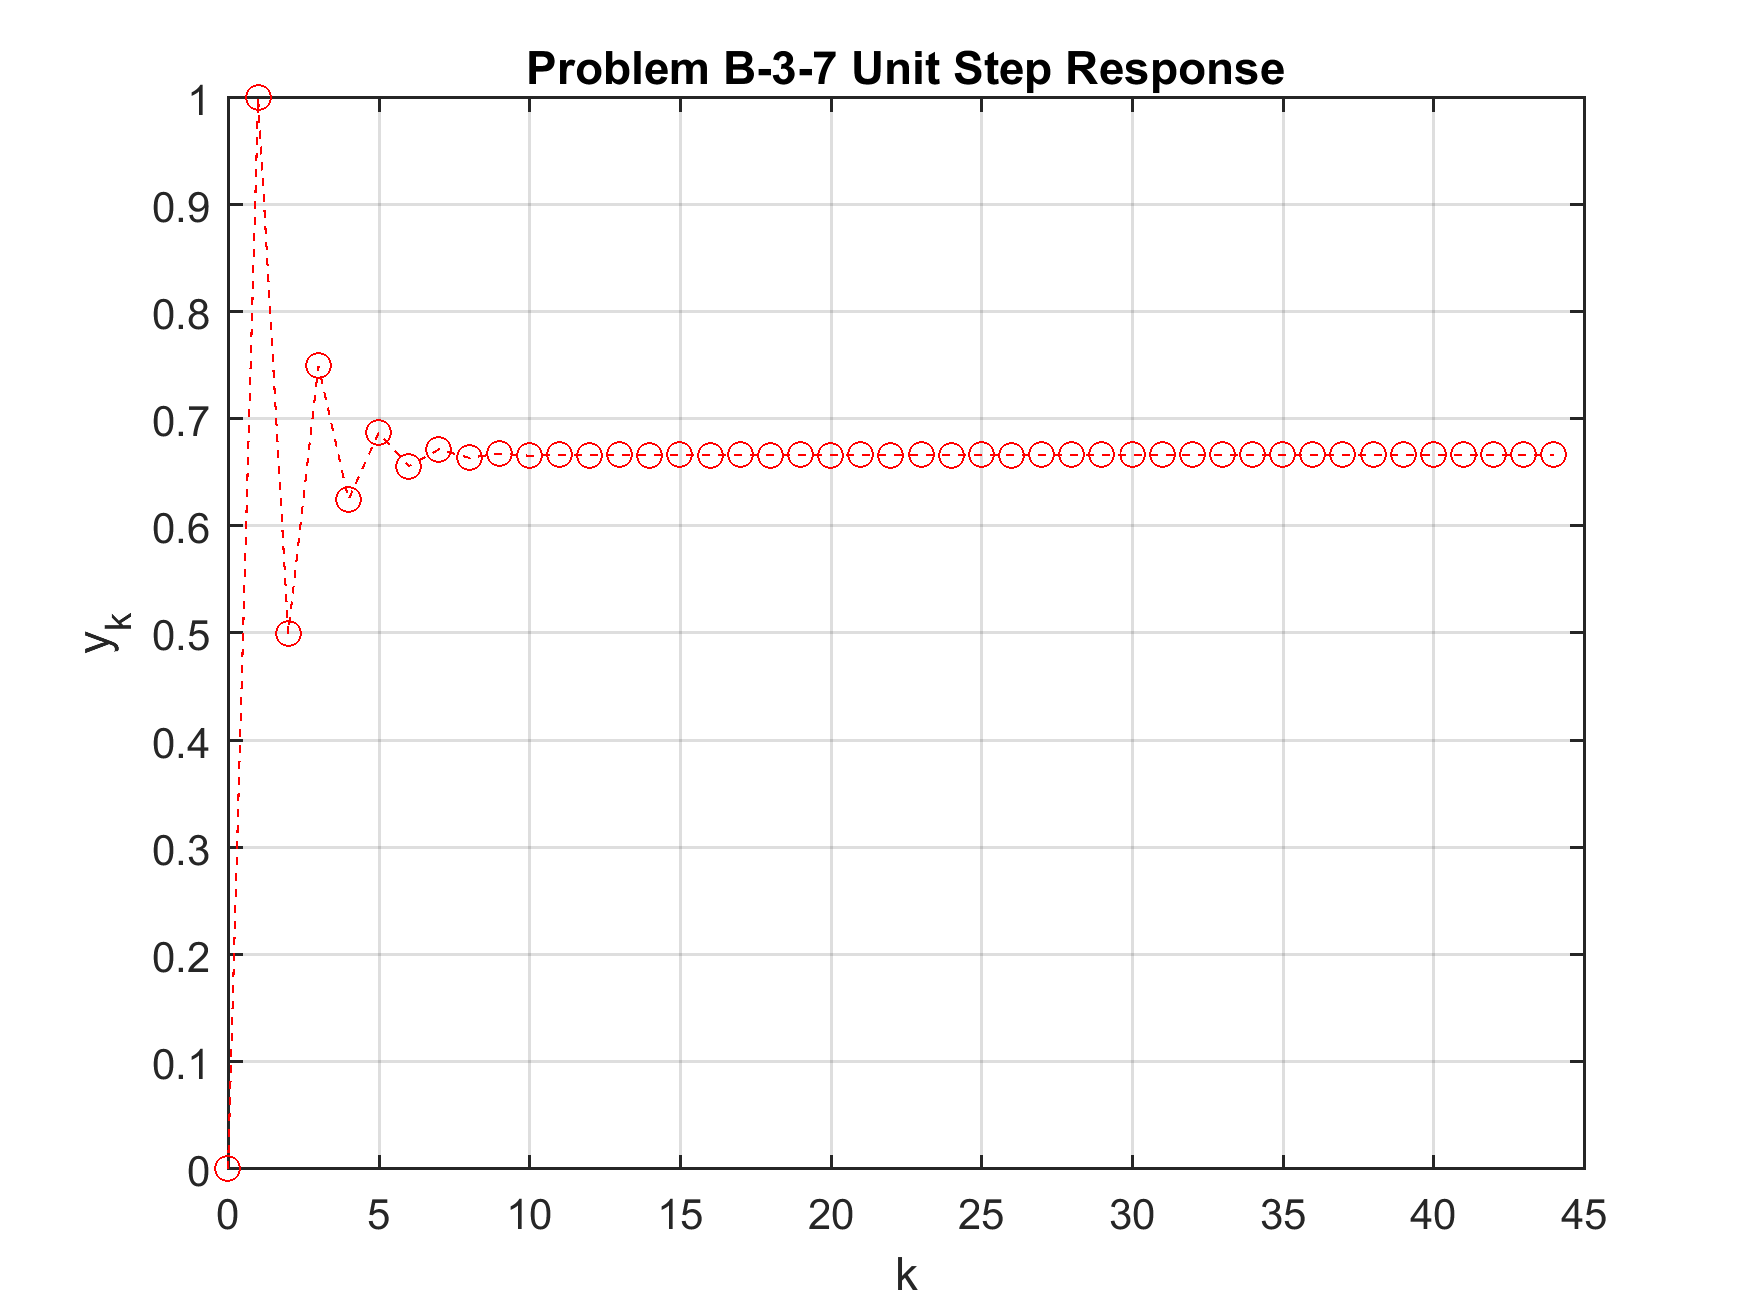
\includegraphics[width=1\linewidth]{PB-3-7}
\end{minipage}


\vspace*{1cm}
\subsection*{B-3-15}



  %     \begin{par}
Obtain the closed-loop pulse transfer function of the system shown in the figure below.
%\end{par} \vspace{1em}
%\begin{par}

\begin{figure}[H]
	\centering
	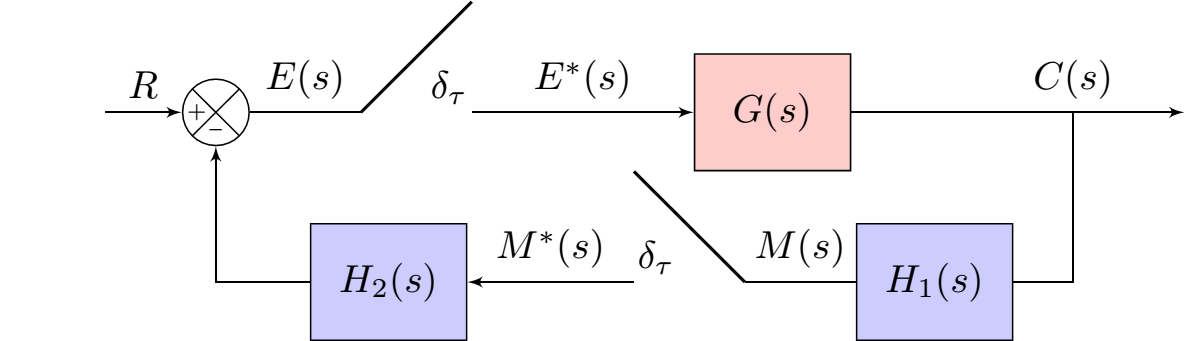
\includegraphics [width=0.85\linewidth]{samplerTesting.png}
	\caption{Block Diagram for Figure B-3-15}
	\label{fig:OgataB-3-15}
	%\caption{}
	% Alternative is to typeset the caption myself, which makes more sense to me.
	% \label{fig:$OgataB-3-15.png$}
\end{figure}
\vspace*{-1cm}
% See http://web.cecs.pdx.edu/~tymerski/ece452/Chapter3.pdf
\begin{align*}
& E (s) = R(s)- H_2(s)M^\ast(s) \quad C(s)= G(s)E^\ast(s)  \quad M(s)=H_1(s)C(s)=H_1(s)G(s) E^\ast(s) 
\end{align*}
% https://en.wikipedia.org/wiki/Starred_transform
Taking the starred Laplace transforms leads to:
\begin{align}
& E^\ast(s)=R^\ast(s)-H_2^\ast M^\ast(s) \\
& C^\ast(s) = G^\ast(s)E^\ast(s) \\ 
& M^\ast(s)= [GH_1(s)]^\ast  E^\ast(s)
\end{align}

Using equations (1) and (3), the
\begin{align} 
& E^\ast = R^\ast(s)-H_2^\ast ([GH_1(s)]^\ast  E^\ast(s)) \\
& E^\ast = \frac{R^\ast(s)}{H_2^\ast [GH_1(s)]^\ast }
\end{align}
Using equation (2) and (5)
\begin{align*}
& C^\ast(s) =  \frac{G^\ast(s)R^\ast(s)}{H_2^\ast [GH_1(s)]^\ast }\\
& H_{\text{transfer}}^\ast(s)=\frac{C^\ast(s)}{R^\ast(s)} = \frac{G^\ast(s)}{H_2^\ast [GH_1(s)]^\ast } \\
& H_{\text{transfer}}^\ast(z)= \frac{G(z)}{H_2(z) [GH_1(z)]}
\end{align*}
\subsection*{B-3-17}

\begin{figure}[H]
	\centering
	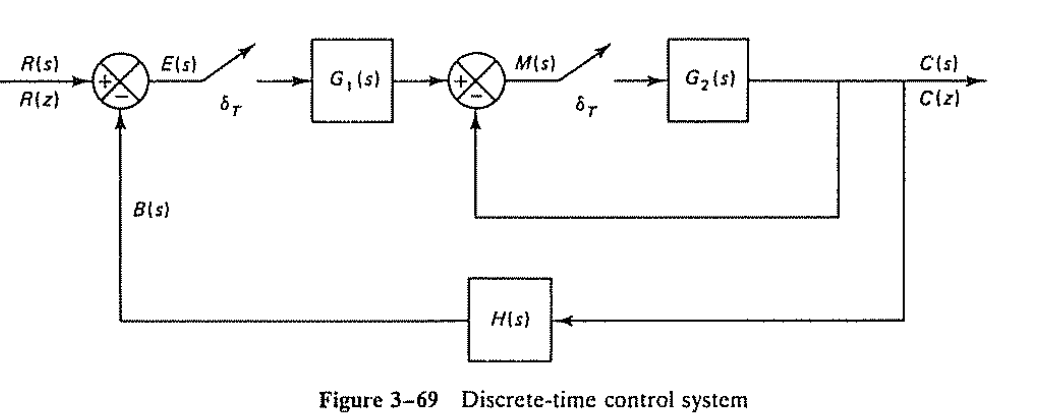
\includegraphics [width=0.85\linewidth]{OgataB-3-17.png}
	%\caption{$OgataB-3-17.png$}
	%\caption{}
	% Alternative is to typeset the caption myself, which makes more sense to me.
	% \label{fig:$OgataB-3-17.png$}
\end{figure}

\begin{align*}
& E (s) = R(s)- H(s)C(s) = R(s) - H(s)G_2(s)M^\ast(s) \\
& C(s)= G_2(s)M^\ast(s)  \\
& M(s)=G_1(s) E^\ast(s) - G_2(s)M^\ast(s)
\end{align*}

Taking the starred Laplace Transform of equations 

\begin{align}
& E^\ast(s)=R^\ast(s)-[G_2H(s)]^\ast M^\ast(s) \\
& C^\ast(s) = G_2^\ast(s)M^\ast(s) \\
& M^\ast(s)=G_1^\ast(s) E^\ast(s) -G_2^\ast (s) M^\ast(s)
\end{align}

Using equations (6) and (8)
\begin{align}
&  M^\ast(s)=G_1^\ast(s) \left\{ R^\ast(s)-[G_2H(s)]^\ast M^\ast(s) \right\} - G_2^\ast (s) M^\ast(s) \\
&  M^\ast(s) \left[1 +G_2^\ast(s)+G_1^\ast(s) \left[G_2H(s)\right]^\ast\right]=G_1^\ast(s)R^\ast(s) \\
&  M^\ast(s) = \frac{G_1^\ast(s)R^\ast(s)}{1 +G_2^\ast(s)+G_1^\ast(s) \left[G_2H(s)\right]^\ast}
\end{align}

Using equations (11) and (7)

\begin{align*}
& C^\ast(s) = \frac{G_2^\ast(s)G_1^\ast(s)R^\ast(s)}{1 +G_2^\ast(s)+G_1^\ast(s) \left[G_2H(s)\right]^\ast} \quad  C(z) =  \frac{R(z)G_2(z) G_1(z)}{1 +G_2(z)+G_1(z) \left[G_2H(z)\right]} %\\
%&\frac{C^\ast(s)}{R^\ast(s)} = \frac{  G_2^\ast(s) G_1^\ast(s)R^\ast(s)}{1 +G_2^\ast(s)+G_1^\ast(s) \left[G_2H(s)\right]^\ast}&  \frac{1}{R^\ast(s)}  = 
%\frac{  G_2^\ast(s) G_1^\ast(s)}{1 +G_2^\ast(s)+G_1^\ast(s) \left[G_2H(s)\right]^\ast} \\
%& & \frac{C(z)}{R(z)} = \frac{  G_2(z) G_1(z)}{1 +G_2(z)+G_1(z) \left[G_2H(z)\right]}  \\
\end{align*}
\end{document}
    
